\documentclass[10pt]{beamer}
%%% Pour le français %%%
\usepackage[utf8]{inputenc}
\usepackage[T1]{fontenc}
\usepackage[frenchb]{babel}
%%%%%%%%%%%%%%%%%%%%%%%%
% \usepackage{fancyhdr} % En-tête et pied de page personnalisés
% \usepackage{listings} % Pour du beau code coloré
%%%% Pour des maths %%%%
\usepackage{mathtools} % Pour pleins de commandes avec des maths
\usepackage{amssymb} % Pour les symboles
\usepackage{amstext} % Pour utiliser \text
% \usepackage{mathrsfs} % 3 fonts pour les 26 lettres
% \usepackage{amsthm} % Custom des theoremes
% \usepackage{tikz} % Pour des graphiques
\usepackage{stmaryrd} % Pour les double crochets, parenthèses etc..
%%%%%%%%%%%%%%%%%%%%%%%%
% \usepackage{layout} % Pour afficher le gabarit de mise en page
% \usepackage{geometry} % Pour régler les marges
% \usepackage{setspace} % Pour modifier l'interligne
% \usepackage{ulem} % Pour souligner et barrer du texte
%%% Pour des polices %%%
% \usepackage{bookman}
% \usepackage{charter}
% \usepackage{newcent}
% \usepackage{lmodern}
% \usepackage{mathpazo}
% \usepackage{mathptmx}
%%%%%%%%%%%%%%%%%%%%%%%%
% \usepackage{url} % Pour citer des urls
% \usepackage{graphicx} % Pour travailler sur des images
% \usepackage{color} % Pour manipuler les couleurs et colorer le texte
\usepackage{enumitem}
\usepackage{tabulary}

\title[TIPE — Transport Optimal]{TIPE \\ Transport Optimal}

\author{ROCHER Kilian — WILLEM Logan}
\date{2020 / 2021}

\mode<presentation>

\useoutertheme[footline=authortitle,subsection=false]{miniframes}
\useinnertheme{circles}
\usecolortheme{whale}
\usecolortheme{orchid}

\definecolor{beamer@blendedblue}{rgb}{0.137,0.466,0.741}
\definecolor{titleColor}{RGB}{102,153,255}
\definecolor{textColor}{RGB}{60,60,60}
\definecolor{frametitlec}{RGB}{17,59,94}

\setbeamercolor{titlelike}{bg=titleColor}
\setbeamercolor{titlelike}{parent=structure}
\setbeamercolor{title}{fg=black}
\setbeamercolor{item}{fg=black}
\setbeamercolor{normal text}{fg=textColor}
\setbeamertemplate{background canvas}[vertical shading][top=cyan!7!white,bottom=cyan!2!white]
\setbeamertemplate{blocks}[rounded][shadow=true]
\setbeamercolor{prop_low}{bg=red!10,fg=black!90}
\setbeamercolor{prop_up}{fg=white,bg=red!90}
\setbeamercolor{data_low}{bg=gray!10,fg=black!90}
\setbeamercolor{data_up}{fg=white,bg=gray!90}

\setbeamercolor{frametitle}{fg=white,bg=frametitlec!95}

\setbeamerfont{frametitle}{size=\small}

\setbeamertemplate{navigation symbols}{%
\insertslidenavigationsymbol % Icône slide
\insertframenavigationsymbol % Icône frame
\insertsubsectionnavigationsymbol % Icône sous section
\insertsectionnavigationsymbol % Icône section
}

\begin{document}
	\begin{frame}[plain]
		\maketitle
	\end{frame}

	\begin{frame}[plain]
		\tableofcontents
	\end{frame}

	\section{Transport optimal}
	
	\subsection{L'optimisation des transports}
	
	\begin{frame}
		\frametitle{L'optimisation des transports}
		Définition de l'optimisation des transports
		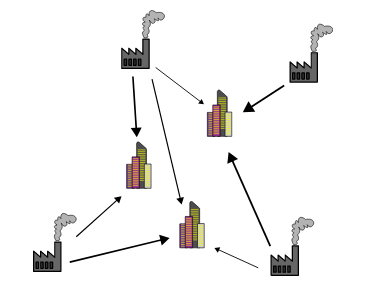
\includegraphics[scale=0.5]{Resultats/Transport_optimal.png}
	\end{frame}
	
	\subsection{Quelques exemples}
	
	\begin{frame}
		\frametitle{Quelques exemples}
		\underline{Quelques problèmes d'optimisation}
		\pause
		\begin{itemize}[label=—]
			\item \textbf{Le voyageur de commerce}
		\end{itemize}
		\ \\
		\begin{center}
			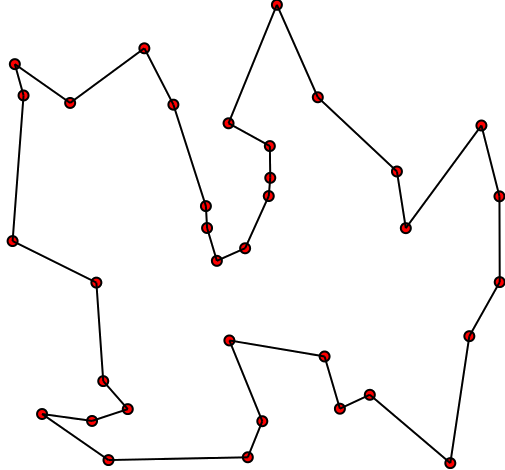
\includegraphics[height=4.5cm,width=4.5cm]{Resultats/voyageur_de_commerce.png}
		\end{center}
	\end{frame}

	\begin{frame}
		\frametitle{Quelques exemples}
		\underline{Quelques problèmes d'optimisation}
		\begin{itemize}[label=—]
			\item Le voyageur de commerce
			\item \textbf{Tournée des véhicules}
		\end{itemize}
		\begin{center}
			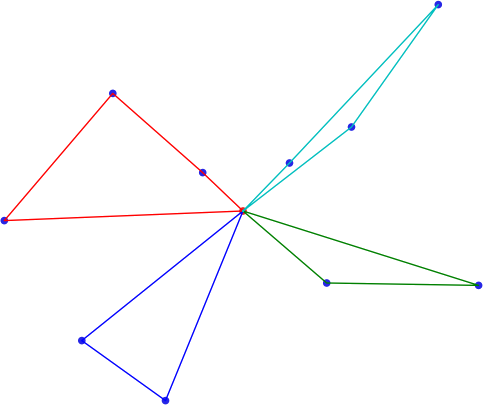
\includegraphics[height=4.5cm,width=4.5cm]{Resultats/tournee_des_vehicules.png}
		\end{center}
	\end{frame}

	\subsection{Applications réelles}

	\begin{frame}
		\frametitle{Applications réelles}
		\begin{figure}
			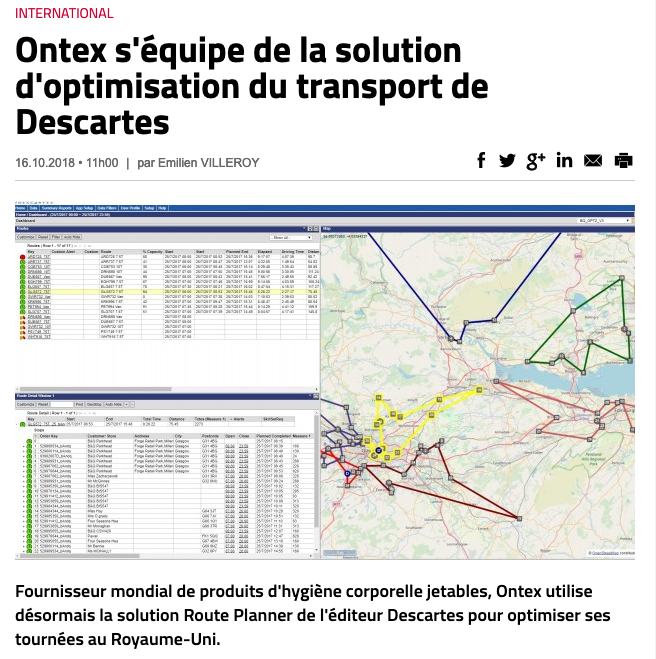
\includegraphics[scale=0.3]{Exemple_concret.png}
		\end{figure}		
	\end{frame}
	
	\section{Problème de tournée des véhicules}

	\subsection{Contexte}
	
	\begin{frame}
		\frametitle{Contexte}
		Dans ce type de problèmes, il s'agit de minimiser le coût total (en distance par exemple) de la tournée de tous les véhicules, ayant pour objectif de livrer à un nombre défini de clients.
		\begin{center}
			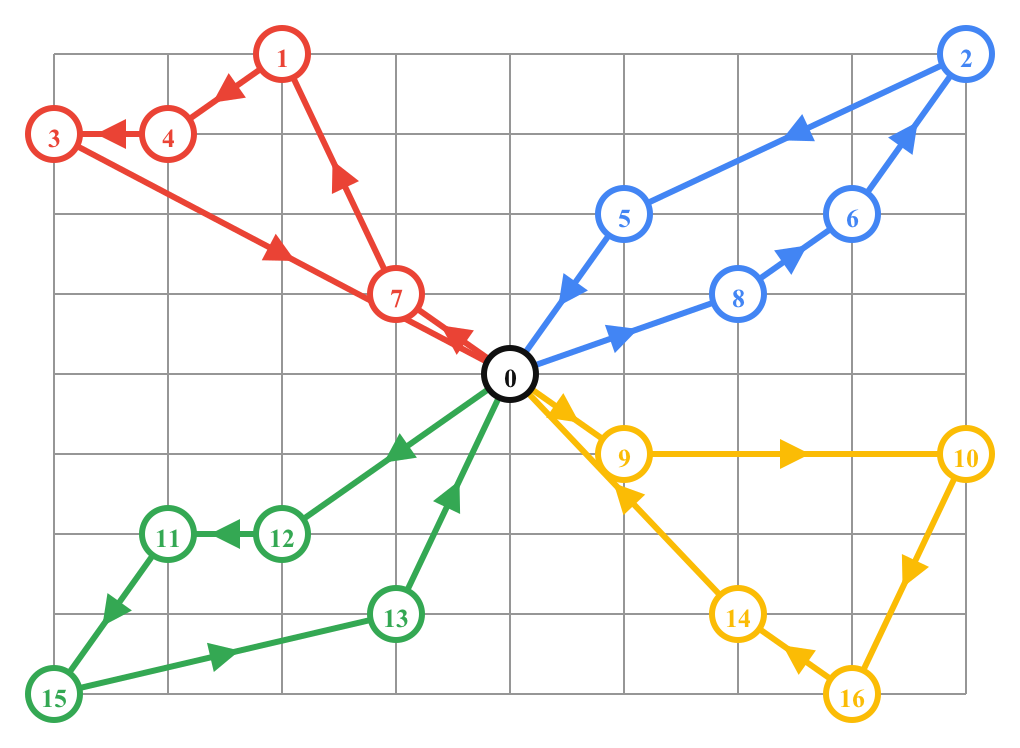
\includegraphics[scale=0.25]{Resultats/vrp.png}
		\end{center}
	\end{frame}

	\subsection{Variantes}
	
	\begin{frame}
		\frametitle{Variantes}
		\underline{Différentes variantes du problème de tournée des véhicules}
		\begin{itemize}[label=—]
			\item Classique (VRP)\pause
			\item Contrainte de capacité (CVRP)\pause
			\item Dépôts multiples (MDVRP)\pause
			\item Retours des colis (VRPPD et VRPB)\pause
			\item \dots 
		\end{itemize}
		\ \newline On s'est intéressé à la version classique afin de s'approprier au mieux le problème.
	\end{frame}
	
	\subsection{Pourquoi utiliser une résolution approchée ?}

	\begin{frame}
		\frametitle{Pourquoi utiliser une résolution approchée ?}
		Deux choix pour le \underline{premier} camion pour chaque client: "OUI" ou "NON"
		\pause
		\begin{center}
			$2^n$ possibilités
		\end{center}
		\pause
		Le sens importe peu:
		\begin{center}
			$2^{n-1}$ possibilités
		\end{center}
		\pause
		\ \\Pour \underline{tous} les trajets, il existe \underline{au moins} $2^{n-1}$ possibilités: \pause 
		\begin{center}
			complexité \textbf{exponentielle}
		\end{center}
	\end{frame}

	\section{Première résolution}

	\subsection{L'algorithme de Clarke \& Wright}

	\begin{frame}
		\frametitle{L'algorithme de Clarke \& Wright}
		\begin{beamerboxesrounded}[upper=data_up,lower=data_low,shadow=true]{Données}
			\begin{itemize}[label=-]
				\item Un point $D$ de coordonnées $(0,0)$ : le dépot
				\pause
				\item Une famille de points \((i_1,...,i_n) \in {(\lbrack-100,100\rbrack^2)}^n\) pour un certain $n \in \lbrack2,+\infty\lbrack$ représentant les clients
				\pause
				\item Une fonction $d$ qui calcule la distance entre deux points.
				\pause
			\end{itemize}
		\end{beamerboxesrounded}\ \newline
		\underline{Remarque} : Dans cette méthode de résolution, le nombre de véhicules n'est pas fixé. C'est l'algorithme qui décide du nombre optimal de véhicules à utiliser. 
	\end{frame}
	 
	\begin{frame}
		\frametitle{L'algorithme de Clarke \& Wright}
		\begin{definition}[Fonction \textit{gain}]
			Fonction $s$ : calcule le gain après raccord de deux routes. \\Pour deux points $i$ et $j$, $s$ calcule la différence de distance entre le chemin \\$D-i-D$ + $D-j-D$ qui vaut $2d(D,i) + 2d(j,D)$ au chemin\\$D-i-j-D$ de distance $d(D,i) + d(i,j) + d(j,D)$
		\begin{align*}
			s(i,j) &= 2d(D,i) + 2d(j,D) - \lbrack d(D,i) + d(i,j) + d(j,D)\rbrack \\
			s(i,j) &= d(D,i) + d(j,D) - d(i,j)
		\end{align*}
		\end{definition}
		\pause
		\begin{tabular}{cccc}
			\;\;\;\;\;\;\;
			&
			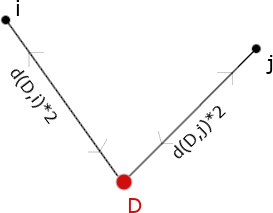
\includegraphics[scale=1.5]{did+djd.png}
			&
			\;\;\;\;\;\;\;	
			\pause		
			&
			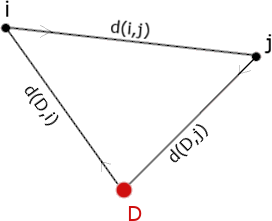
\includegraphics[scale=1.5]{dijd.png}			
		\end{tabular}
	\end{frame}

   \begin{frame}
	\frametitle{L'algorithme de Clarke \& Wright}
		\underline{L'algorithme comporte deux étapes majeures}
		\begin{itemize}[label=—]
			\item \textbf{Étape 1: Calcul des bénéfices}
			\ \\ Calcul la liste des bénéfices $s_{ij}$ pour $i,j \in \llbracket 1,n \rrbracket$ et tri de cette liste
		\end{itemize}
		\begin{center}
			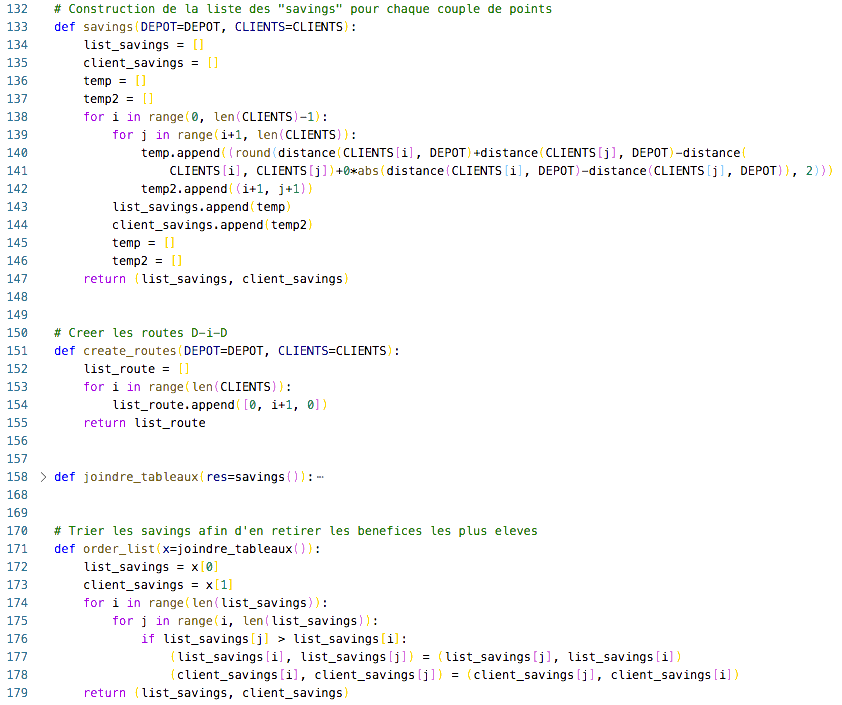
\includegraphics[scale=0.25]{Resultats/Etape_1.png}
		\end{center}
	\end{frame}

	\begin{frame}
		\frametitle{L'algorithme de Clarke \& Wright}
		\underline{L'algorithme comporte deux étapes majeures}
		\begin{itemize}[label=—]
			\item Étape 1: Calcul des bénéfices
			\ \\ Calcul la liste des bénéfices $s_{ij}$ pour $i,j \in \llbracket 1,n \rrbracket$ et tri de cette liste
			\item \textbf{Etape 2: Fusion des routes}
			\ \\ Fusion des routes si celles-ci peuvent l'être, dans l'ordre donné par la liste précédente
		\end{itemize}
		\begin{center}
			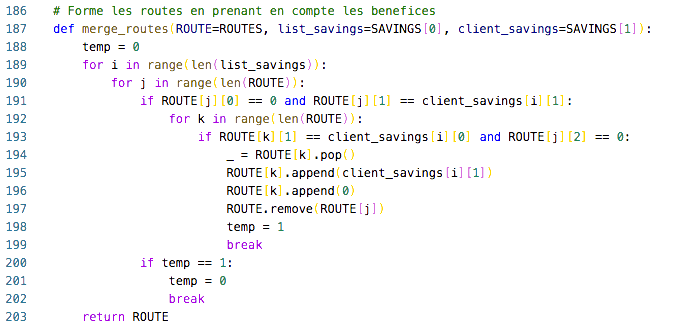
\includegraphics[scale=0.3]{Resultats/Etape_2.png}
		\end{center}
	\end{frame}

	\subsection{Résultat}

	\begin{frame}
		\frametitle{Résultat}
		\begin{figure}
			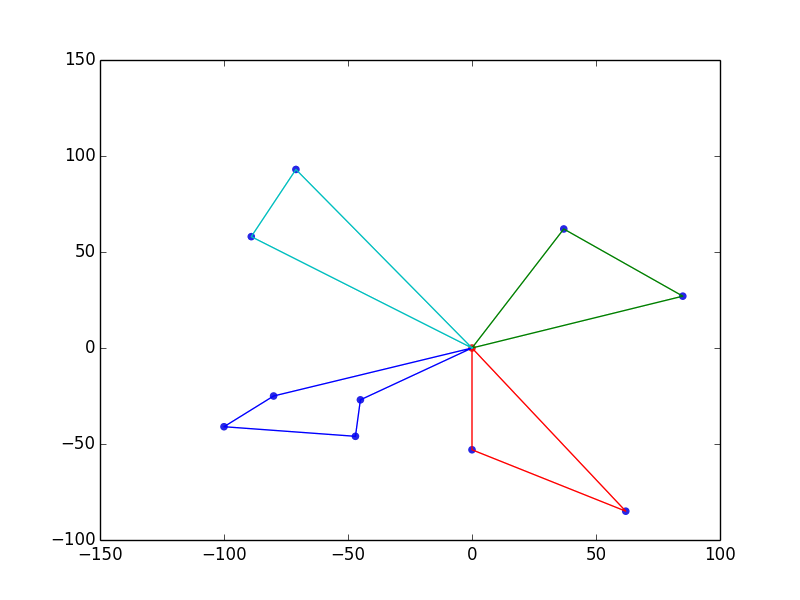
\includegraphics[scale=0.35]{Resultats/CasParfait.png}
			\caption{Solution satisfaisante d'un problème}	
		\end{figure}
	\end{frame}

	\subsection{Insuffisance de l'algorithme}
	   
	\begin{frame}
		\frametitle{Insuffisance de l'algorithme}
		\begin{figure}
			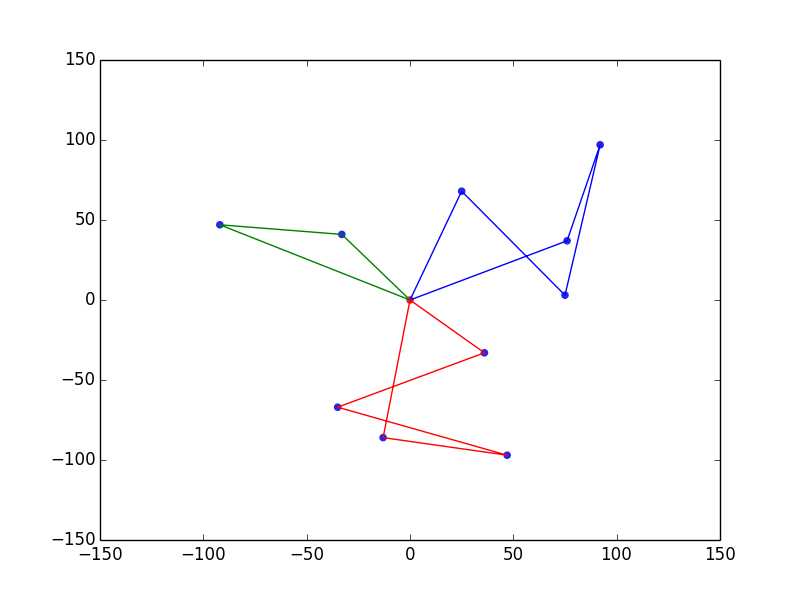
\includegraphics[scale=0.35]{Resultats/Cas_avant_2-opt.png}
			\caption{Résultat non satisfaisant pour 10 clients}	
		\end{figure}
	\end{frame}

	\begin{frame}
		\frametitle{Insuffisance de l'algorithme}
		\begin{figure}
			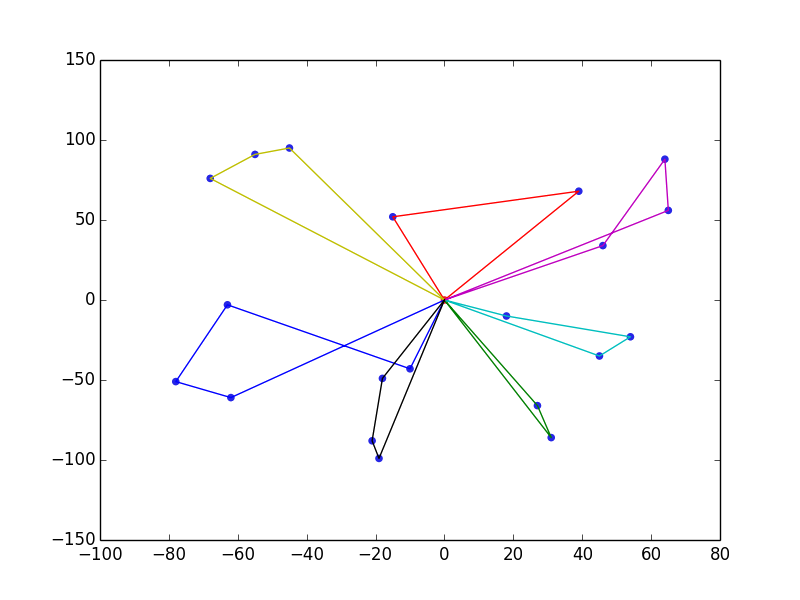
\includegraphics[scale=0.35]{Resultats/Cas_avant_2-opt3_distance_totale_1442,4672107499957.png}
			\caption{Résultat non satisfaisant pour 20 clients}	
		\end{figure}
	\end{frame}

	\section{Amélioration}

	\subsection{Le 2-opt}

	\begin{frame}
		\frametitle{Le 2-opt}
		\begin{tabular}{cc}
				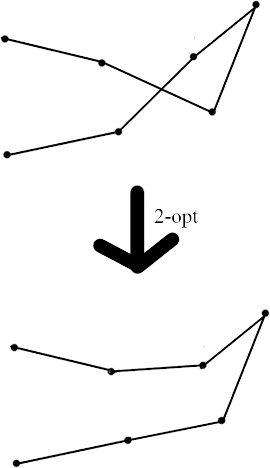
\includegraphics[scale=1.1]{Resultats/principe-2-opt.png}
				&
				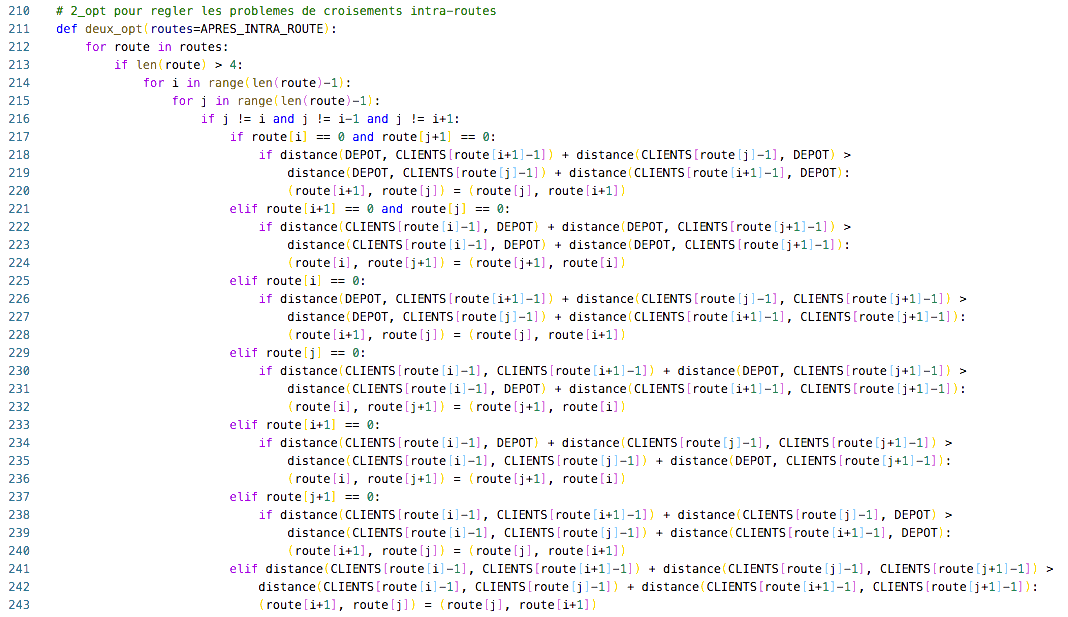
\includegraphics[scale=0.2]{Resultats/2opt.png}
				\\
				\ \\Principe du 2-opt\\Suppression des liaisons sécantes
				&
				Vue générale de l'algorithme
		\end{tabular}
	\end{frame}

	\subsection{Résultats avec 2-opt}
	
	\begin{frame}
		\frametitle{Résultats avec 2-opt}
		\begin{center}
		\textbf{10 clients}
		\end{center}
		\ \newline
		\begin{tabular}{cc}
			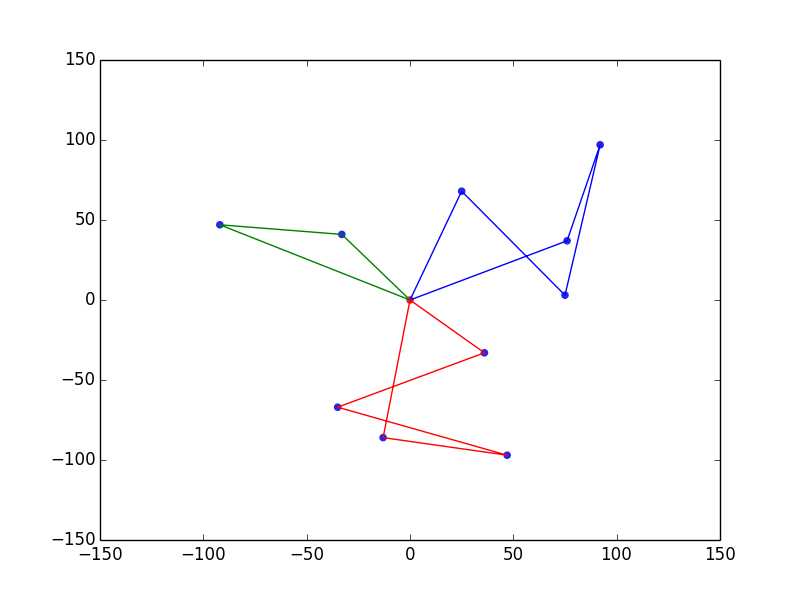
\includegraphics[scale=0.25]{Resultats/Cas_avant_2-opt.png}
			&
			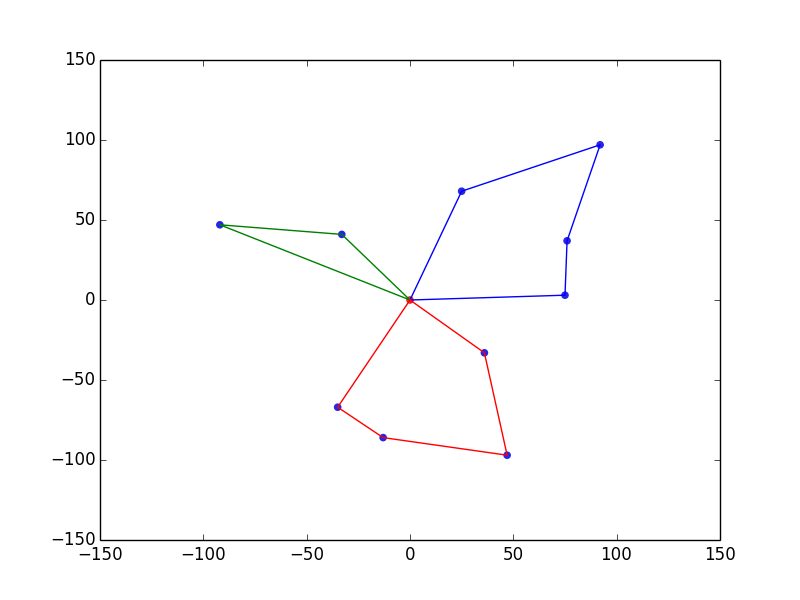
\includegraphics[scale=0.25]{Resultats/Cas_apres_2-opt.png}
			\\                                                     
			Avant&Après
		\end{tabular}
	\end{frame}
	
	\begin{frame}
		\frametitle{Résultats avec 2-opt}
		\begin{center}
			\textbf{20 clients}
		\end{center}
		\ \newline
		\begin{tabular}{cc}
			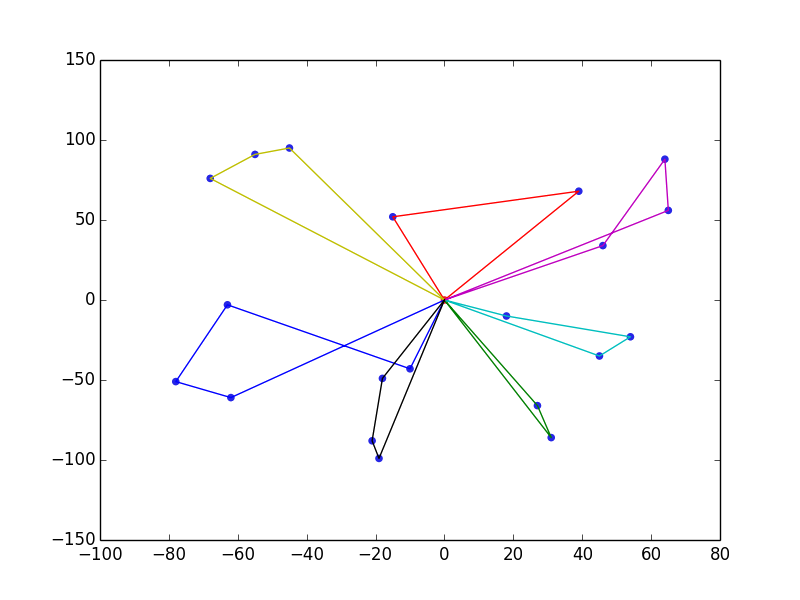
\includegraphics[scale=0.25]{Resultats/Cas_avant_2-opt3_distance_totale_1442,4672107499957.png}
			&
			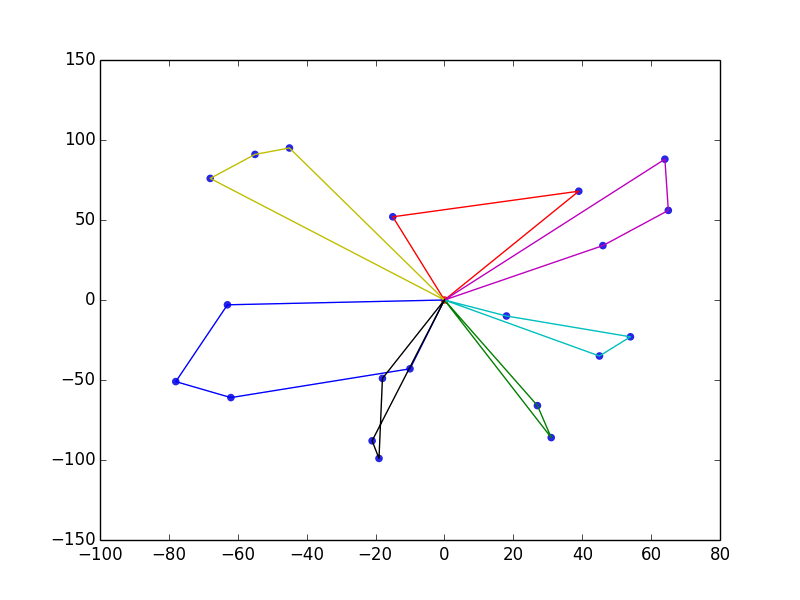
\includegraphics[scale=0.25]{Resultats/Cas_apres_2-opt3_distance_totale_1402,9109633508515.png}
			\\
			Distance: 1442km&Distance: 1403km
			\\                                                     
			Avant&Après
		\end{tabular}
	\end{frame}
	
	\subsection{Complexité des algorithmes}

	\begin{frame} 
		\frametitle{Complexité des algorithmes}
		\begin{tabular}{cc}
			\textbf{Sans 2-opt}&\textbf{Avec 2-opt}
			\\
			\ &\
			\\
			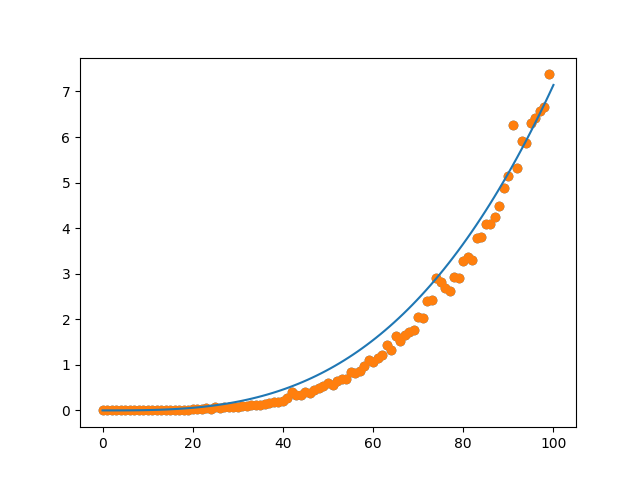
\includegraphics[scale=0.3]{Resultats/Complexite_algo_Clarke_and_Wright_x3_140000_sans_2opt.png}
			&
			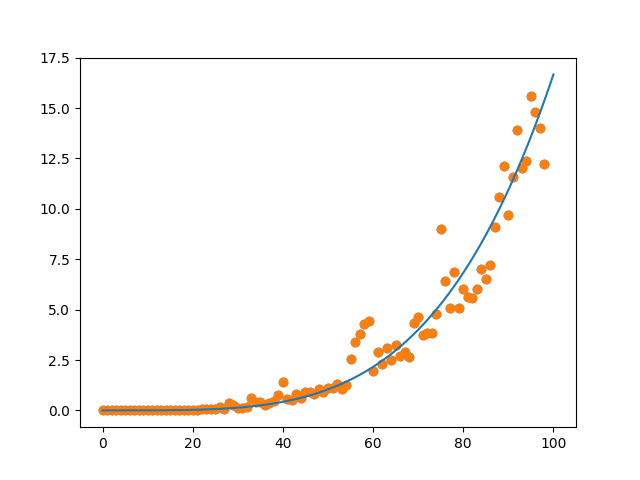
\includegraphics[scale=0.3]{Resultats/Complexite_algo_Clark_and_Wright_x4_6000000.png}
			\\
			\small{$f(x) = x^3/14000$}&\small{$f(x) = x^4/6000000$}
		\end{tabular}
	\end{frame}

	\subsection{Limite de l'algorithme ?}

	\begin{frame}
		\frametitle{Limite de l'algorithme ?}
		Mauvaise résolution pour les points suivants: \ \\
		\begin{center}
			$i_1 = (20, 0)$, $i_2 = (-16, -12)$, $i_3 = (16, -12)$
		\end{center}
		\pause
		\begin{tabular}{cc}
			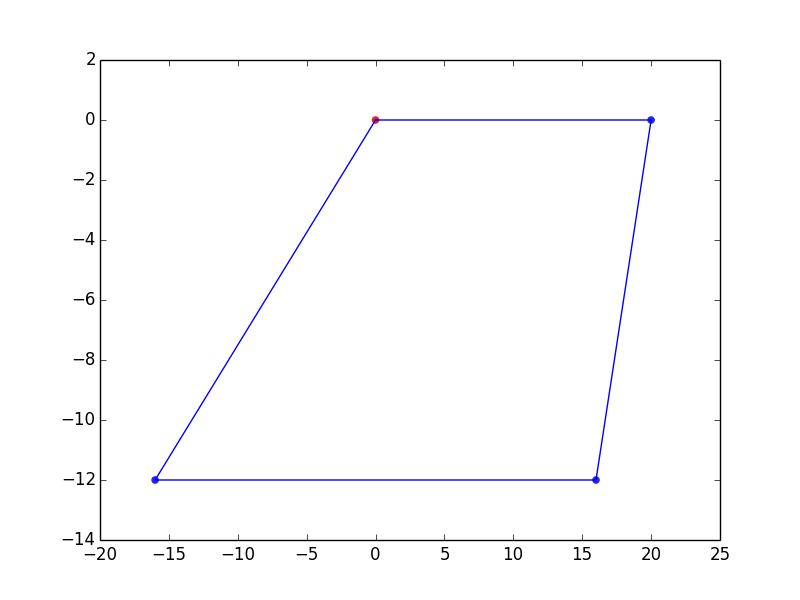
\includegraphics[scale=0.25]{Resultats/Cas_defavorable_avant_2opt.png}
			&
			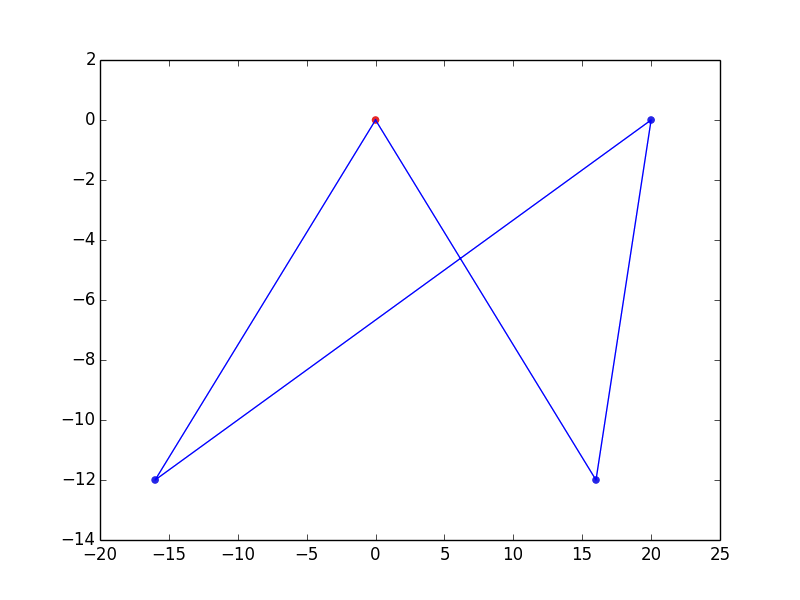
\includegraphics[scale=0.25]{Resultats/Cas_defavorable_2opt.png}
			\\
			Distance: 85km&Distance: 91km
			\\
			Avant 2-opt&Après 2-opt
		\end{tabular}
	\end{frame}

\end{document}